\documentclass[12pt, letterpaper]{article}
\usepackage[english]{babel}
\usepackage[margin=1in]{geometry}
%\usepackage[utf8]{inputenc} 				% This code is old, it may not work for some users. 
\usepackage{abstract, adjustbox, amsmath, amssymb, array, indentfirst, fancyhdr, floatrow, listings, longtable, multicol, multirow, natbib, parskip, pdflscape, setspace, tabu, tabularx, tikz, titlesec, verbatim, xcolor}
\usepackage{wrapfig, lipsum}
\usepackage{booktabs}
\usepackage{tabularx}
\usepackage{rotating}
\usepackage{pdfpages}
\usepackage{indentfirst}
\usepackage[format=plain,up,textfont=normal,up,justification=centering,singlelinecheck=false]{caption}   
\usepackage[bottom]{footmisc}
\pagestyle{fancy}
\fancyhead[C]{\rule{.5\textwidth}{4\baselineskip}} % Add a BIG header
\setlength{\headheight}{22pt}
\lstset{basicstyle=\ttfamily, columns=flexible, breaklines=true}
\fancyhf{}
\PassOptionsToPackage{hyphens}{url}
\usepackage[colorlinks=false, hidelinks]{hyperref}
\lhead{\footnotesize{Course Title \\ Author Name}}
\rhead{\footnotesize{Assignment Name \\ \today}} % alternatively delete \today and write out the date
\renewcommand{\headrulewidth}{1pt}
\fancyfoot[C]{\footnotesize\thepage}
\newcolumntype{R}{>{\raggedright\arraybackslash}X}
\titleformat{\section}{\large\bfseries}{\thesection}{1em}{} 
\floatsetup[figure]{capposition=top}
\floatsetup[table]{capposition=top} 
%\onehalfspacing
%\doublespacing
\singlespacing

\begin{document} 
\bibliographystyle{Chicago16} 	%Make sure to download the bibliography style before you compile
\setcitestyle{aysep={}}
%\tableofcontents 
%\listoftables
%\listoffigures

\setlength{\parindent}{0.85cm}
\subparagraph{1.} 
\noindent \\ The variable XYZ is a nominal variable, which can be seen in Table \ref{t1}.

\begin{table}[ht]\caption{Age Frequency Distribution Table}\label{t1}
	\centering
	\begin{tabular}{lrrr}
		\hline
		Age & Frequency & Percent & Valid Percent \\ 
		\hline
		1 & 652 & 15.27 & 15.71 \\ 
		2 & 761 & 17.82 & 18.34 \\ 
		3 & 620 & 14.52 & 14.94 \\ 
		4 & 781 & 18.29 & 18.82 \\ 
		5 & 769 & 18.01 & 18.53 \\ 
		6 & 567 & 13.28 & 13.66 \\ 
		NA's & 121 & 2.83 &  \\ 
		\hline
		Total & 4271 & 100.00 & 100.00 \\ 
		\hline
	\end{tabular}
\end{table}

\pagebreak

\begin{figure}\caption{Density Curves of 2012 State Voter Turnout and 2012 State Cigarette Taxes}\label{f3}
	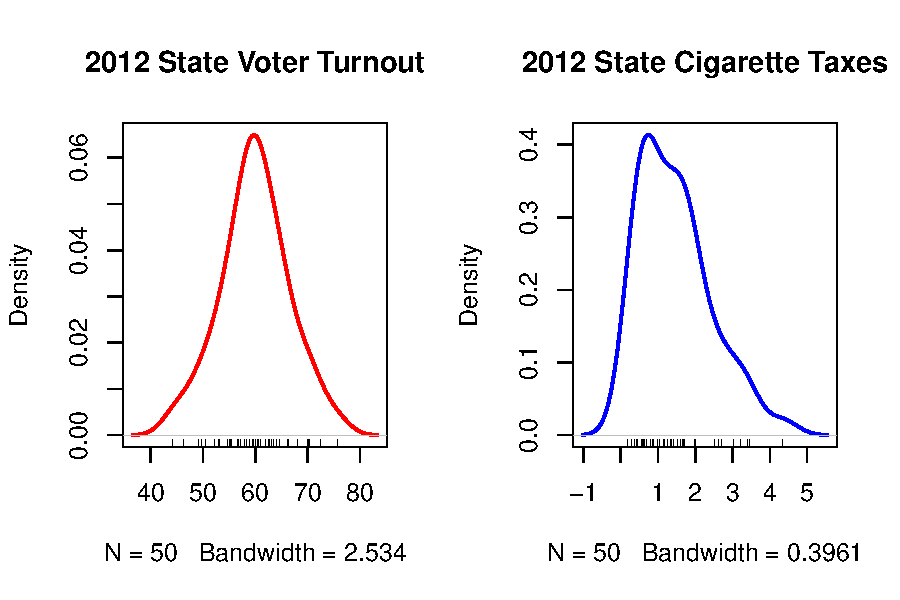
\includegraphics[scale=.9]{votecigsden.pdf}
\end{figure}

\end{document}